\documentclass{beamer}
%% Possible paper sizes: a0, a0b, a1, a2, a3, a4.
%% Possible orientations: portrait, landscape
%% Font sizes can be changed using the scale option.
\usepackage[size=a3,orientation=landscape,scale=3.75]{beamerposter}
\usetheme{LLT-poster}
%\usecolortheme{ComingClean}
\usecolortheme{Entrepreneur}
%\usecolortheme{ConspicuousCreep}  %% VERY garish.
\usepackage{graphicx}
\usepackage{xcolor, colortbl}
\usepackage{array}

\def\mybar#1{%%
    #1 & {\color{red}\pgfmathsetlengthmacro\x{#1*0.006mm}\rule{\x}{4pt}}}
\usepackage[utf8]{inputenc}
\usepackage[T1]{fontenc}
\usepackage{libertine}
\usepackage[scaled=0.92]{inconsolata}
\usepackage[libertine]{newtxmath}
\usepackage{geometry}
\geometry{paperwidth=32in,paperheight=40in,margin=3cm}
\usepackage{multicol}
\usepackage{mwe}

\author[mvn5218@psu.edu]{Markus Neumann}
\title{Government websites as data: A methodological pipeline with application to the websites of municipalities in the United States \\ \vspace{10mm} \small{Markus Neumann,  Fridolin Linder,  Bruce Desmarais \\ Department of Political Science - Penn State University}}
\institute{The Pennsylvania State University}
% Optional foot image
%\footimage{\includegraphics[width=4cm]{IMG_1934.jpg}}

\begin{document}
\beamertemplatenavigationsymbolsempty
\begin{frame}[fragile]
\begin{columns}[T]

%%%% 1st Column
\begin{column}{.4\textwidth}

\begin{block}{Overview}
\begin{itemize}
\item Websites of local governments are an important source of information for citizens
\item Extant research of government websites has largely relied on manual coding
\item We develop a methodological pipeline for the automated analysis of government websites
\item We demonstrate the use of this pipeline on the websites of 234 municipal websites in CA, IN, LA, NY, TX and WA. 
\item We show that content varies with the partisanship of the mayor.
\end{itemize}
\end{block}

\begin{block}{Data Collection}
\begin{itemize}
\item Scraping city URLs from Wikipedia and the General Services Administration, which keeps a list of all .gov addresses
\item Verification of which websites actually work through an automated browser
\item Downloading the websites through \texttt{wget}
\item Information on mayoral partisanship from state websites, the LEAP project, Ballotpedia and Wikipedia
%\item 234 Websites in CA, IN, LA, NY, TX and WA.
\end{itemize}
\end{block}

\begin{block}{Site to Text Conversion}
\begin{itemize}
\item The file endings from open data sources such as governmental websites are sometimes wrong. This causes problems when converting to text.
\item We use file signatures to identify the correct type before conversion with \texttt{readtext}.
\item Used file types: Html, xml, pdf, doc, docx, txt
\item Everything is converted to .txt
\item Preprocessing: Lowercase; removal of punctuation, numbers, dates, etc.; spellchecking/Removal of non-English words; Lemmatization
\end{itemize}
\end{block}

\begin{block}{Boilerplate Removal}
\begin{itemize}
\item Websites contain a lot of text that is not substantively interesting
\item This text is often repeated on each page of a site - for example website elements such as ``You are here'', ''Home'', or the names of city officials and offices.
\item If this content is not removed, the tool of analysis will associate specific patterns of boilerplate with the respective cities
\item Problem: how to remove boilerplate content without dropping useful information?
\end{itemize}
\end{block}

\begin{block}{Boilerplate Classifier}
\begin{itemize}
\item Solution: Train a classifier (random forest) on manually annotated lines of website content. A line can be flagged as either substantively useful or boilerplate.
\item The classifier relies on the following features:
\begin{itemize}
\item Line length (number of words & characters)
\item Number of line duplications within a website
\item Line position in the document (median distance of a line to the document midpoint)
\end{itemize}
\end{itemize}
\end{block}

\end{column}

%\begin{column}{.63\textwidth}
%\begin{block}{Additional Preprocessing}
%\begin{itemize}
%\item Lowercase; removal of punctuation, numbers, dates, etc.
%\item Spellchecking/Removal of non-English words
%\item Lemmatization
%\end{itemize}
%\end{block}
%\end{column}

%%%% 2nd Column

\begin{column}{.6\textwidth}

%\begin{column}{.23\textwidth}





%\end{column}


%%%%  3rd column

%\begin{column}{.23\textwidth}

\begin{block}{Analysis}

\begin{center}
\begin{itemize}
\item Structural topic model with 60 topics
\item Covariates: Party, state, population, median income
\end{itemize}

\vspace{5mm}

% latex table generated in R 3.4.4 by xtable 1.8-2 package
% Fri Aug 10 15:33:35 2018
\begin{table}[ht]
\centering
\begingroup\footnotesize
\begin{tabular}{rllllllll}
  \hline
 \# & Top Word 1 & Top Word 2 & Top Word 3 & Top Word 4 & Top Word 5 & Top Word 6 & \multicolumn{2}{c}{Tokens assigned} \\ 
  \hline
   42 & \cellcolor{red!20}breastfeed & \cellcolor{red!20}vaccine & \cellcolor{red!20}infection & \cellcolor{red!20}symptom & \cellcolor{red!20}asthma & \cellcolor{red!20}mosquito & \mybar{2497} \\ 
   17 & \cellcolor{red!20}alarm & \cellcolor{red!20}disaster & \cellcolor{red!20}fire & \cellcolor{red!20}rescue & \cellcolor{red!20}preparedness & \cellcolor{red!20}evacuation & \mybar{989} \\ 
   53 & \cellcolor{red!20}drinking & \cellcolor{red!20}wastewater & \cellcolor{red!20}water & \cellcolor{red!20}pipeline & \cellcolor{red!20}pump & \cellcolor{red!20}disinfection & \mybar{461} \\ 

   49 & \cellcolor{red!10}bin & \cellcolor{red!10}recycling & \cellcolor{red!10}garbage & \cellcolor{red!10}recyclables & \cellcolor{red!10}recyclable & \cellcolor{red!10}bag & \mybar{1791} \\ 
    7 & \cellcolor{red!10}energy & \cellcolor{red!10}garland & \cellcolor{red!10}renewable & \cellcolor{red!10}solar & \cellcolor{red!10}electricity & \cellcolor{red!10}climate & \mybar{742} \\ 
   23 & \cellcolor{red!10}bid & \cellcolor{red!10}proposer & \cellcolor{red!10}bidder & \cellcolor{red!10}contractor & \cellcolor{red!10}subcontractor & \cellcolor{red!10}contract & \mybar{447} \\ 
   57 & \cellcolor{red!10}duct & \cellcolor{red!10}conduit & \cellcolor{red!10}bolt & \cellcolor{red!10}splice & \cellcolor{red!10}valve & \cellcolor{red!10}fitting & \mybar{1373} \\ 
   13 & \cellcolor{red!10}server & \cellcolor{red!10}wireless & \cellcolor{red!10}software & \cellcolor{red!10}telecommunication & \cellcolor{red!10}subscriber & \cellcolor{red!10}desktop & \mybar{1092} \\ 
    1 & \cellcolor{red!10}storm & \cellcolor{red!10}runoff & \cellcolor{red!10}infiltration & \cellcolor{red!10}discharge & \cellcolor{red!10}drainage & \cellcolor{red!10}drain & \mybar{516} \\ 
   38 & \cellcolor{red!10}youth & \cellcolor{red!10}student & \cellcolor{red!10}parent & \cellcolor{red!10}teacher & \cellcolor{red!10}immigrant & \cellcolor{red!10}literacy & \mybar{714} \\ 
   59 & \cellcolor{red!10}sampling & \cellcolor{red!10}sample & \cellcolor{red!10}analytical & \cellcolor{red!10}concentration & \cellcolor{red!10}hydrocarbon & \cellcolor{red!10}toxicity & \mybar{1241} \\ 
   45 & \cellcolor{red!10}premise & \cellcolor{red!10}licensee & \cellcolor{red!10}violation & \cellcolor{red!10}license & \cellcolor{red!10}permit & \cellcolor{red!10}inspection & \mybar{509} \\ 
   60 & \cellcolor{red!10}exhaust & \cellcolor{red!10}fugitive & \cellcolor{red!10}aircraft & \cellcolor{red!10}airport & \cellcolor{red!10}aviation & \cellcolor{red!10}diesel & \mybar{731} \\ 
   %30 & \cellcolor{white}fort & \cellcolor{white}thence & \cellcolor{white}blvd & \cellcolor{white}worth & \cellcolor{white}ave & \cellcolor{white}west & \mybar{681} \\ 
   %58 & \cellcolor{white}councilor & \cellcolor{white}auburn & \cellcolor{white}plain & \cellcolor{white}ward & \cellcolor{white}beech & \cellcolor{white}glen & \mybar{480} \\ 
   %51 & \cellcolor{white}whereas & \cellcolor{white}councilman & \cellcolor{white}alderman & \cellcolor{white}ordain & \cellcolor{white}hereby & \cellcolor{white}resolution & \mybar{420} \\ 
   %16 & \cellcolor{white}recreation & \cellcolor{white}park & \cellcolor{white}golf & \cellcolor{white}playground & \cellcolor{white}picnic & \cellcolor{white}zoo & \mybar{682} \\ 
   %36 & \cellcolor{white}retiree & \cellcolor{white}retirement & \cellcolor{white}actuarial & \cellcolor{white}deductible & \cellcolor{white}dental & \cellcolor{white}pension & \mybar{470} \\ 
   %27 & \cellcolor{white}exam & \cellcolor{white}incumbent & \cellcolor{white}supervise & \cellcolor{white}supervision & \cellcolor{white}examination & \cellcolor{white}knowledge & \mybar{687} \\ 
   %56 & \cellcolor{white}historic & \cellcolor{white}landmark & \cellcolor{white}revival & \cellcolor{white}archaeological & \cellcolor{white}century & \cellcolor{white}historian & \mybar{2587} \\ 
   %12 & \cellcolor{white}parking & \cellcolor{white}hotel & \cellcolor{white}garage & \cellcolor{white}space & \cellcolor{white}retail & \cellcolor{white}square & \mybar{321} \\ 
   %41 & \cellcolor{white}tax & \cellcolor{white}exemption & \cellcolor{white}abatement & \cellcolor{white}real & \cellcolor{white}estate & \cellcolor{white}property & \mybar{310} \\ 
    4 & \cellcolor{white}facade & \cellcolor{white}awning & \cellcolor{white}porch & \cellcolor{white}roof & \cellcolor{white}balcony & \cellcolor{white}exterior & \mybar{1108} \\ 

   15 & \cellcolor{blue!10}complainant & \cellcolor{blue!10}defendant & \cellcolor{blue!10}allegation & \cellcolor{blue!10}complaint & \cellcolor{blue!10}allege & \cellcolor{blue!10}discrimination & \mybar{1384} \\ 
 
   14 & \cellcolor{blue!10}yes & \cellcolor{blue!10}agency & \cellcolor{blue!10}federal & \cellcolor{blue!10}recipient & \cellcolor{blue!10}compliance & \cellcolor{blue!10}entity & \mybar{205} \\ 

   25 & \cellcolor{blue!10}cannabis & \cellcolor{blue!10}marijuana & \cellcolor{blue!10}senate & \cellcolor{blue!10}dispensary & \cellcolor{blue!10}ballot & \cellcolor{blue!10}cultivation & \mybar{1188} \\ 

   47 & \cellcolor{blue!10}employee & \cellcolor{blue!10}overtime & \cellcolor{blue!10}sick & \cellcolor{blue!10}wage & \cellcolor{blue!10}grievance & \cellcolor{blue!10}bargaining & \mybar{511} \\ 

   37 & \cellcolor{blue!10}audit & \cellcolor{blue!10}auditor & \cellcolor{blue!10}internal & \cellcolor{blue!10}procedure & \cellcolor{blue!10}accountability & \cellcolor{blue!10}oversight & \mybar{420} \\ 
   21 & \cellcolor{blue!10}housing & \cellcolor{blue!10}affordable & \cellcolor{blue!10}homeless & \cellcolor{blue!10}homelessness & \cellcolor{blue!10}affordability & \cellcolor{blue!10}landlord & \mybar{318} \\ 
   34 & \cellcolor{blue!10}comment & \cellcolor{blue!10}draft & \cellcolor{blue!10}feedback & \cellcolor{blue!10}stakeholder & \cellcolor{blue!10}suggest & \cellcolor{blue!10}discussion & \mybar{289} \\ 
   19 & \cellcolor{blue!10}debt & \cellcolor{blue!10}bond & \cellcolor{blue!10}governmental & \cellcolor{blue!10}obligation & \cellcolor{blue!10}financial & \cellcolor{blue!10}accounting & \mybar{251} \\ 
   40 & \cellcolor{blue!10}bicycle & \cellcolor{blue!10}bike & \cellcolor{blue!10}lane & \cellcolor{blue!10}crosswalk & \cellcolor{blue!10}pedestrian & \cellcolor{blue!10}bicyclist & \mybar{574} \\ 
   32 & \cellcolor{blue!20}budget & \cellcolor{blue!20}revenue & \cellcolor{blue!20}expenditure & \cellcolor{blue!20}appropriation & \cellcolor{blue!20}fund & \cellcolor{blue!20}million & \mybar{242} \\ 
   48 & \cellcolor{blue!20}absent & \cellcolor{blue!20}aye & \cellcolor{blue!20}khan & \cellcolor{blue!20}nay & \cellcolor{blue!20}berry & \cellcolor{blue!20}voting & \mybar{528} \\ 
   31 & \cellcolor{blue!20}chair & \cellcolor{blue!20}agenda & \cellcolor{blue!20}commission & \cellcolor{blue!20}speaker & \cellcolor{blue!20}chairperson & \cellcolor{blue!20}committee & \mybar{314} \\ 
   55 & \cellcolor{blue!80}robbery & \cellcolor{blue!80}homicide & \cellcolor{blue!80}arrest & \cellcolor{blue!80}sergeant & \cellcolor{blue!80}suspect & \cellcolor{blue!80}burglary & \mybar{1395} \\ 
   \hline
\end{tabular}
\endgroup
%\caption{Top words from a structural topic model with 60 topics and FREX scoring. Colors depict partisanship based on coefficient size. White cells are non-significant topics.} 
\label{tabSTMtopwords60}
\end{table}



%\begin{figure}
%    \centering
%    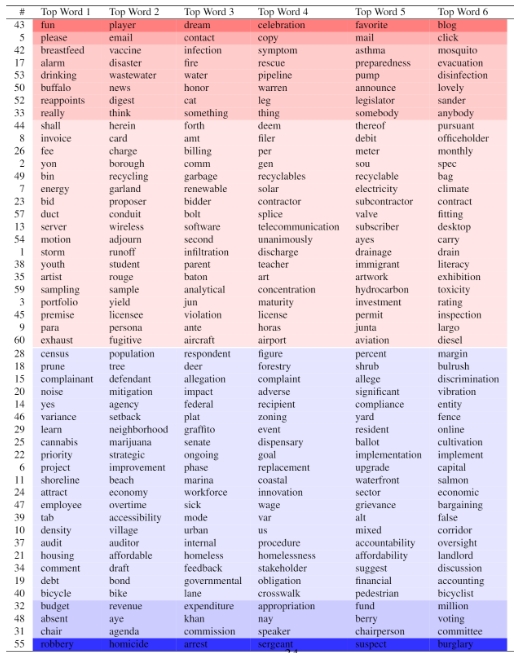
\includegraphics[width=\linewidth]{stm_test.png}
%    %\caption{Caption}
%    \label{fig:my_label}
%\end{figure}

\end{center}

\end{block}

\begin{block}{Conclusion}
\begin{itemize}
\item Cities with Republican mayors provide more information about basic utilities such as water, energy, fire safety, or  natural disaster protection.
\item Cities with Democratic mayors provide more information about policy deliberation, crime control, or public housing.
\item These findings call into question the commonly held notion that politics at the municipal level is largely non-partisan.
\item We plan to implement the pipeline in an R package
\end{itemize}
\end{block}

%\end{column}
\end{column}

\end{columns}



\end{frame}
\end{document}